
\langsection[subsection]{Know Your Motorcycle}{Знать свой мотоцикл}

\begin{langblock}{0.425}
\begin{eng}	
	There are plenty of things on the highway that can cause you trouble. Your motorcycle should not be one of them. To make sure that your motorcycle won't let you down:
	\begin{itemize}[noitemsep]
		\item \textbf{Read} owner's manual first.
		\item \textbf{Start} with the right motorcycle for you.
		\item \textbf{Be familiar} with the motorcycle controls.
		\item \textbf{Check} the motorcycle before every ride.
		\item \textbf{Keep} it in safe riding condition between rides.
		\item \textbf{Avoid} add-ons and modifications that make your motorcycle harder to handle.
	\end{itemize}
\end{eng}
\begin{rus}
		На пути может быть множество факторов, которые могут создать проблемы. Ваш мотоцикл не должен стать одним из них. Чтобы убедиться, что мотоцикл не подведет вас:
		\begin{itemize}[noitemsep]
			\item \textbf{Сначала} ознакомьтесь с руководством пользователя.
			\item \textbf{Начните} с подходящего для вас мотоцикла.
			\item \textbf{Изучите} органы управления мотоциклом.
			\item \textbf{Проверяйте} мотоцикл перед каждой поездкой.
			\item \textbf{Поддерживайте} его в безопасном состоянии между поездками.
			\item \textbf{Избегайте} дополнительных аксессуаров и модификаций, которые усложняют управление мотоциклом.
		\end{itemize}
\end{rus}
\end{langblock}









\langsection[subsubsection]{The Right Motorcycle for You}{Мотоцикл который вам подходит}


\begin{langblock}{0.425}
\begin{eng}	
	First, make sure your motorcycle is right for you. It should ``fit`` you. Your feet should reach the ground while you are seated on the motorcycle, and the controls should be easy to operate. Smaller motorcycles are usually easier for beginners to operate.
	
	\textit{At minimum, your street-legal motorcycle should have:}
	\begin{itemize}[noitemsep]
		\bfseries
		\item Headlight, taillight and brakelight.
		\item Front and rear brakes.
		\item Turn signals.
		\item Horn.
		\item Two mirrors.
	\end{itemize}
\end{eng}
\begin{rus}
		Прежде всего убедитесь, что мотоцикл вам подходит. Он должен «соответствовать» вам. Ваши ноги должны доставать до земли, когда вы сидите на мотоцикле, а органы управления должны быть удобны в обращении. Для начинающих обычно легче в управлении мотоциклы меньшего размера.
		
		\textit{Как минимум, ваш мотоцикл должен быть оборудован:}
		\begin{itemize}[noitemsep]
			\bfseries
			\item Передней фарой, задним фонарем и стоп-сигналом.
			\item Передним и задним тормозами.
			\item Указателями поворота.
			\item Звуковым сигналом.
			\item Двумя зеркалами.
		\end{itemize}
\end{rus}
\end{langblock}









\langsection[subsubsection]{Borrowing and Lending}{Мотоцикл на прокат}

\begin{langblock}{0.425}
\begin{eng}	
	Borrowers and lenders of motorcycles, beware. Crashes are fairly common among beginning riders especially in the first months of riding. Riding an unfamiliar motorcycle adds to the problem. If you borrow a motorcycle, get familiar with it in a controlled area. And if you lend your motorcycle to friends, make sure they are licensed and know how to ride before allowing them out into traffic.
	
	No matter how experienced you may be, ride extra carefully on any motorcycle that's new or unfamiliar to you. It takes time to adjust, so give yourself a greater margin for errors.
\end{eng}
\begin{rus}
		Будьте аккуратны с арендой мотоцикла. ДТП довольно часто происходят с начинающими, особенно в первые месяцы езды. Управление незнакомым мотоциклом усугубляет проблему. Если вы берете мотоцикл напрокат, ознакомьтесь с ним на небольшой площадке. Если вы даете свой мотоцикл друзьям, убедитесь, что у них есть водительское удостоверение соответствующей категории и они умеют ездить, прежде чем выпускать их на дорогу. В независимости от вашего опыта, на незнакомо вам мотоцикле рулите с особой осторожностью. Адаптация требует времени, поэтому держите больший запас времени и дистанции на случай ошибки.
\end{rus}
\end{langblock}









\langsection[subsubsection]{Get Familiar with the Motorcycle Controls}{Изучите органы управления}

\begin{langblock}{0.425}
\begin{eng}	
	Make sure you are completely familiar with the motorcycle before you take it out on the street. Be sure to review the owner's manual. This is particularly important if you are riding a borrowed motorcycle. If you are going to use an unfamiliar motorcycle:
	\begin{itemize}
		\item \textbf{Make all the checks} you would on your own motorcycle.
		\item \textbf{Find out where everything is}, particularly the turn signals, horn, headlight switch, fuel-control valve, and engine cut-off switch. Find and operate these items without having to look for them.
		\item Know the gear pattern. Work the throttle, clutch, and brakes a few times before you start riding. All controls react a little differently.
		\item Ride very cautiously and be aware of surroundings. Accelerate gently, take turns more slowly, and leave extra room for stopping.
	\end{itemize}
\end{eng}
\begin{rus}
		Убедитесь, что вы полностью знакомы со своим мотоциклом, прежде чем выезжать на улицу. Обязательно ознакомьтесь с руководством пользователя. Это особенно важно, если вы управляете мотоциклом взятым напрокат. Если вы собираетесь использовать незнакомый мотоцикл:
		\begin{itemize}
			\item \textbf{Выполните все проверки}, которые вы выполняли бы на собственном мотоцикле.
			\item \textbf{Изучите расположение всех органов управления}, особенно указателей поворота, звукового сигнала, переключателя фары, топливного клапана и выключателя зажигания двигателя. Находить и использовать каждый орган управления не глядя на него.
			\item \textbf{Знайте схему переключения передач}. Несколько раз поработайте дроссельной заслонкой, сцеплением и тормозами перед началом движения. Все органы управления реагируют немного по-разному.
			\item \textbf{Езжайте крайне осторожно} и внимательно смотрите по сторонам. Плавно разгоняйтесь, проходите повороты на меньшей скорости и оставляйте дополнительный запас для торможения.
		\end{itemize}
\end{rus}
\end{langblock}

\begin{figure}[htbp]
	\centering
	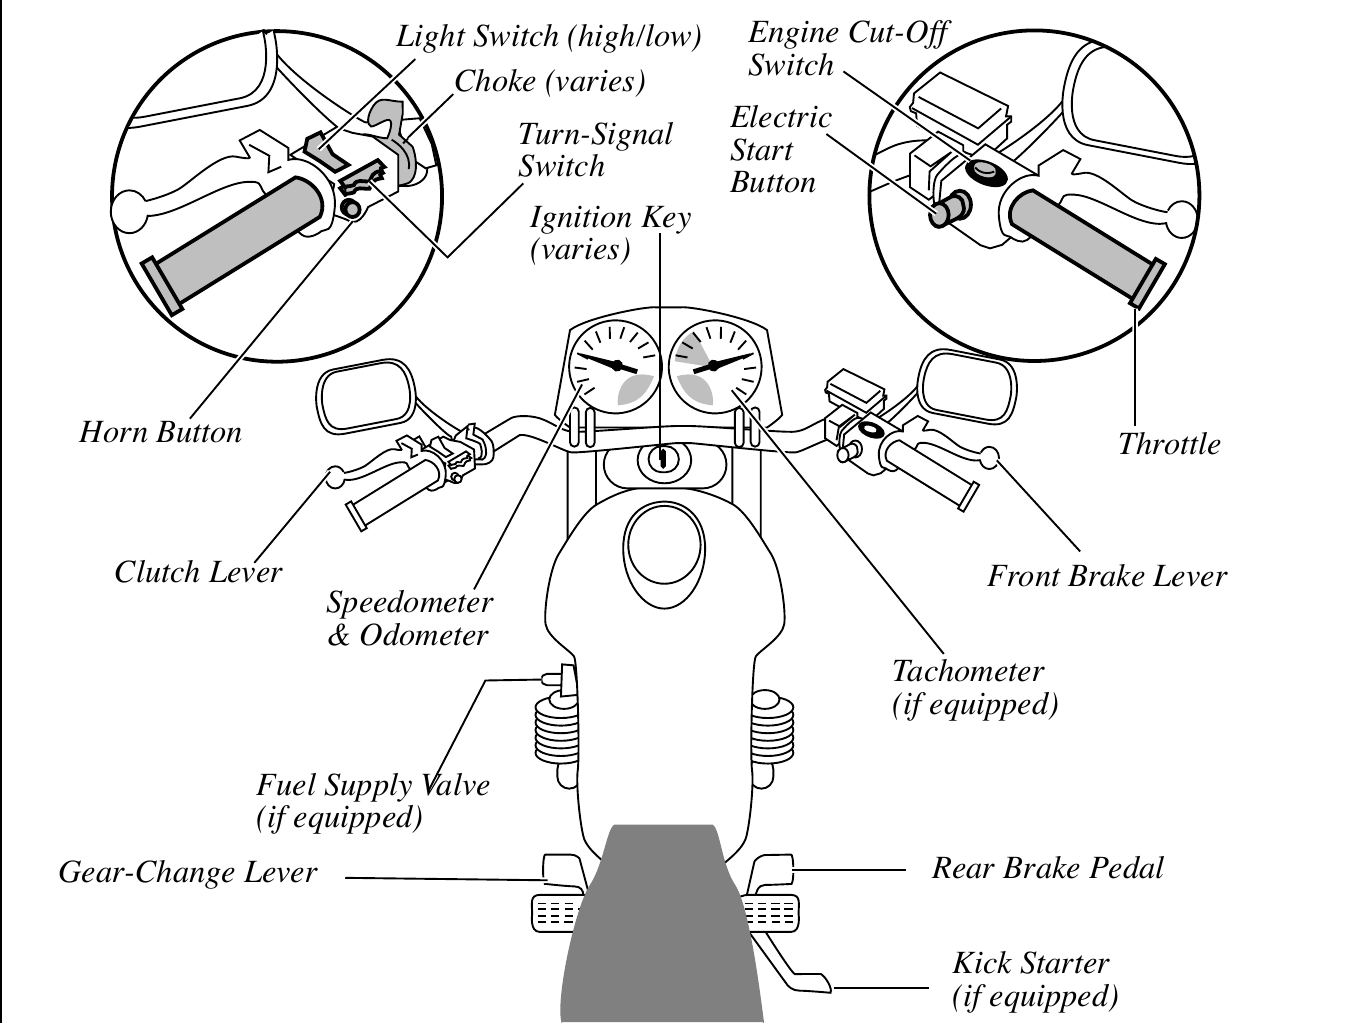
\includegraphics[width=0.95\textwidth, frame]{moto_controls}
	\caption{Motorcycle controls}
	\label{fig:moto_controls}
\end{figure}





\langsection[subsubsection]{Check Your Motorcycle}{Проверка мотоцикла}


\begin{langblock}{0.425}
\begin{eng}	
	A motorcycle needs more frequent attention than a car. A minor technical failure in a car seldom leads to anything more than an inconvenience for the driver.
	If something's wrong with the motorcycle, you'll want to find out about it before you get in traffic. Make a complete check of your motorcycle before every ride.
	\newline\newline
	\textit{Before mounting the motorcycle make the following checks:}
	\begin{itemize}
		\item \textbf{Tires/Wheels} Check the condition of tread, wheels, and air pressure.
		\item \textbf{Fluids} --- Oil and fluid levels. At a minimum, check hydraulic fluids and coolants weekly. Look under the motorcycle for signs of an oil or gas leak.
		\item \textbf{Headlights and Taillight} --- Check them both. Test your switch to make sure both high and low beams are working.
		\item \textbf{Turn Signals} --- Turn on both right and left turn signals. Make sure all lights are working properly.
		\item \textbf{Brake Light} --- Try both brake controls, and make sure each one turns on the brake light.
		\item \textbf{Controls} (levers, cables, throttle) --- Check the condition, operation, and routing.
	\end{itemize}
	Once you have mounted the motorcycle, complete the following checks before starting out:
	\begin{itemize}
		\item \textbf{Clutch and Throttle} --- Make sure they work smoothly. The throttle should snap back when you let go. The clutch should feel tight and smooth.
		\item \textbf{Mirrors} --- Clean and adjust both mirrors before starting. It's difficult to ride with one hand while you try to adjust a mirror. Adjust each mirror so you can see the lane behind and as much as possible of the lane next to you. When properly adjusted, a mirror may show the edge of your arm or shoulder --- but it's the road behind and to the side that's most important.
		\item \textbf{Brakes} --- Try the front and rear brake levers one at a time. Make sure each one feels firm and holds the motorcycle when the brake is fully applied.
		\item \textbf{Horn} --- Try the horn. Make sure it works.
	\end{itemize}
\end{eng}
\begin{rus}
		Мотоцикл требует более частого внимания, чем автомобиль. Незначительная техническая неисправность в автомобиле редко приводит к чему-либо большему, чем просто неудобства для водителя.
		
		Если с мотоциклом что-то не так, то вы захотите узнать об этом до того как окажетесь на дороге. Выполняйте полную проверку мотоцикла перед каждой поездкой.
		\newline\newline
		\textit{Перед тем как сесть на мотоцикл, выполните следующие проверки:}
		\begin{itemize}
			\item \textbf{Шины/колеса} "--- проверьте состояние протектора, колес и давления воздуха.
			\item \textbf{Тормозные жидкости} "--- уровни масла и рабочих жидкостей. Посмотрите под мотоциклом нет ли подтеков масла или бензина. Проверяйте гидравлические и охлаждающую жидкости как минимум раз в неделю. 
			\item \textbf{Передние и задние фонари} "--- проверьте оба. А так же переключатель ближнего и дальнего света.
			\item \textbf{Указатели поворота} "--- проверьте правый и левый указатели поворота. Убедитесь, что все четыре лампы поворотов работают.
			\item \textbf{Стоп-сигнал} "--- проверьте оба тормоза и убедитесь, что каждый включает стоп-сигнал.
			\item \textbf{Органы управления} (рычаги, тросы, дроссельная заслонка) "--- проверьте состояние, работу и крепление.
		\end{itemize}
		После того как вы сели на мотоцикл, выполните следующие проверки перед началом движения:
		\begin{itemize}
			\item \textbf{Сцепление и дроссельная заслонка} "--- убедитесь, что они работают плавно. Дроссельная заслонка должна возвращаться в исходное положение при отпускании. Сцепление должно чувствоваться упругим и плавным.
			\item \textbf{Зеркала} "--- протрите и отрегулируйте оба зеркала перед началом движения. Ехать с одной рукой, пытаясь отрегулировать зеркало, затруднительно. Отрегулируйте каждое зеркало так, чтобы видеть полосу позади и максимально возможную часть соседней полосы. При правильной регулировке в зеркале может быть виден край руки или плеча, но наиболее важна дорога позади и сбоку.
			\item \textbf{Тормоза} "--- испытайте передний и задний тормоз по отдельности. Убедитесь, что каждый работает надежно и удерживает мотоцикл при полном нажатии.
			\item \textbf{Звуковой сигнал} "--- попробуйте звукового сигнала. Убедитесь, что он работает.
		\end{itemize}
\end{rus}
\end{langblock}






